\documentclass[12pt]{article}

% -------------------- Packages --------------------
\usepackage{hyperref}
\usepackage{listings}
\usepackage[margin=1in]{geometry}
\usepackage{enumitem}
\usepackage{array}
\usepackage{titlesec}
\usepackage{helvet}
\renewcommand{\familydefault}{\sfdefault}

% Math packages
\usepackage{amsmath}     % For math equations
\usepackage{amssymb}     % For advanced math symbols
\usepackage{amsfonts}    % For math fonts
\usepackage{gvv}         % Custom matrix/vector formatting
\usepackage{esint}

% Other packages
\usepackage[utf8]{inputenc}
\usepackage{graphicx}
\usepackage{pgfplots}
\pgfplotsset{compat=1.18}
\usepackage{multirow}
\usepackage{float}
\usepackage{caption}
\usepackage{multicol}

% -------------------- Formatting --------------------
\titleformat{\section}{\bfseries\large}{\thesection.}{1em}{}
\setlength{\parindent}{0pt}
\setlength{\parskip}{6pt}
\renewcommand{\labelenumi}{\alph{enumi})}

% -------------------- Document --------------------
\begin{document}

\newpage
\begin{center}
\textbf{\Large AI25BTECH11034 - SUJAL CHAUHAN }\\
\textbf{3.4.3}
\end{center}

\textbf{Question:}\\
Construct a square of side 3 unit
\vspace{1cm}
\textbf{Solution}\\
Let's consider four points A,B,C,D as vertices of square:
\begin{center}
    \begin{tabular}{|c|c|} \hline
       Point  & Positon Vector \\ \hline
       A  & \myvec{0 \\ 0} \\ \hline
       B  & \myvec{3 \\ 0} \\ \hline
       C  & \myvec{3\\ 3} \\ \hline
       D  & \myvec{0 \\ 3} \\ \hline
    \end{tabular}
\end{center}

\begin{figure}[h]
    \centering
    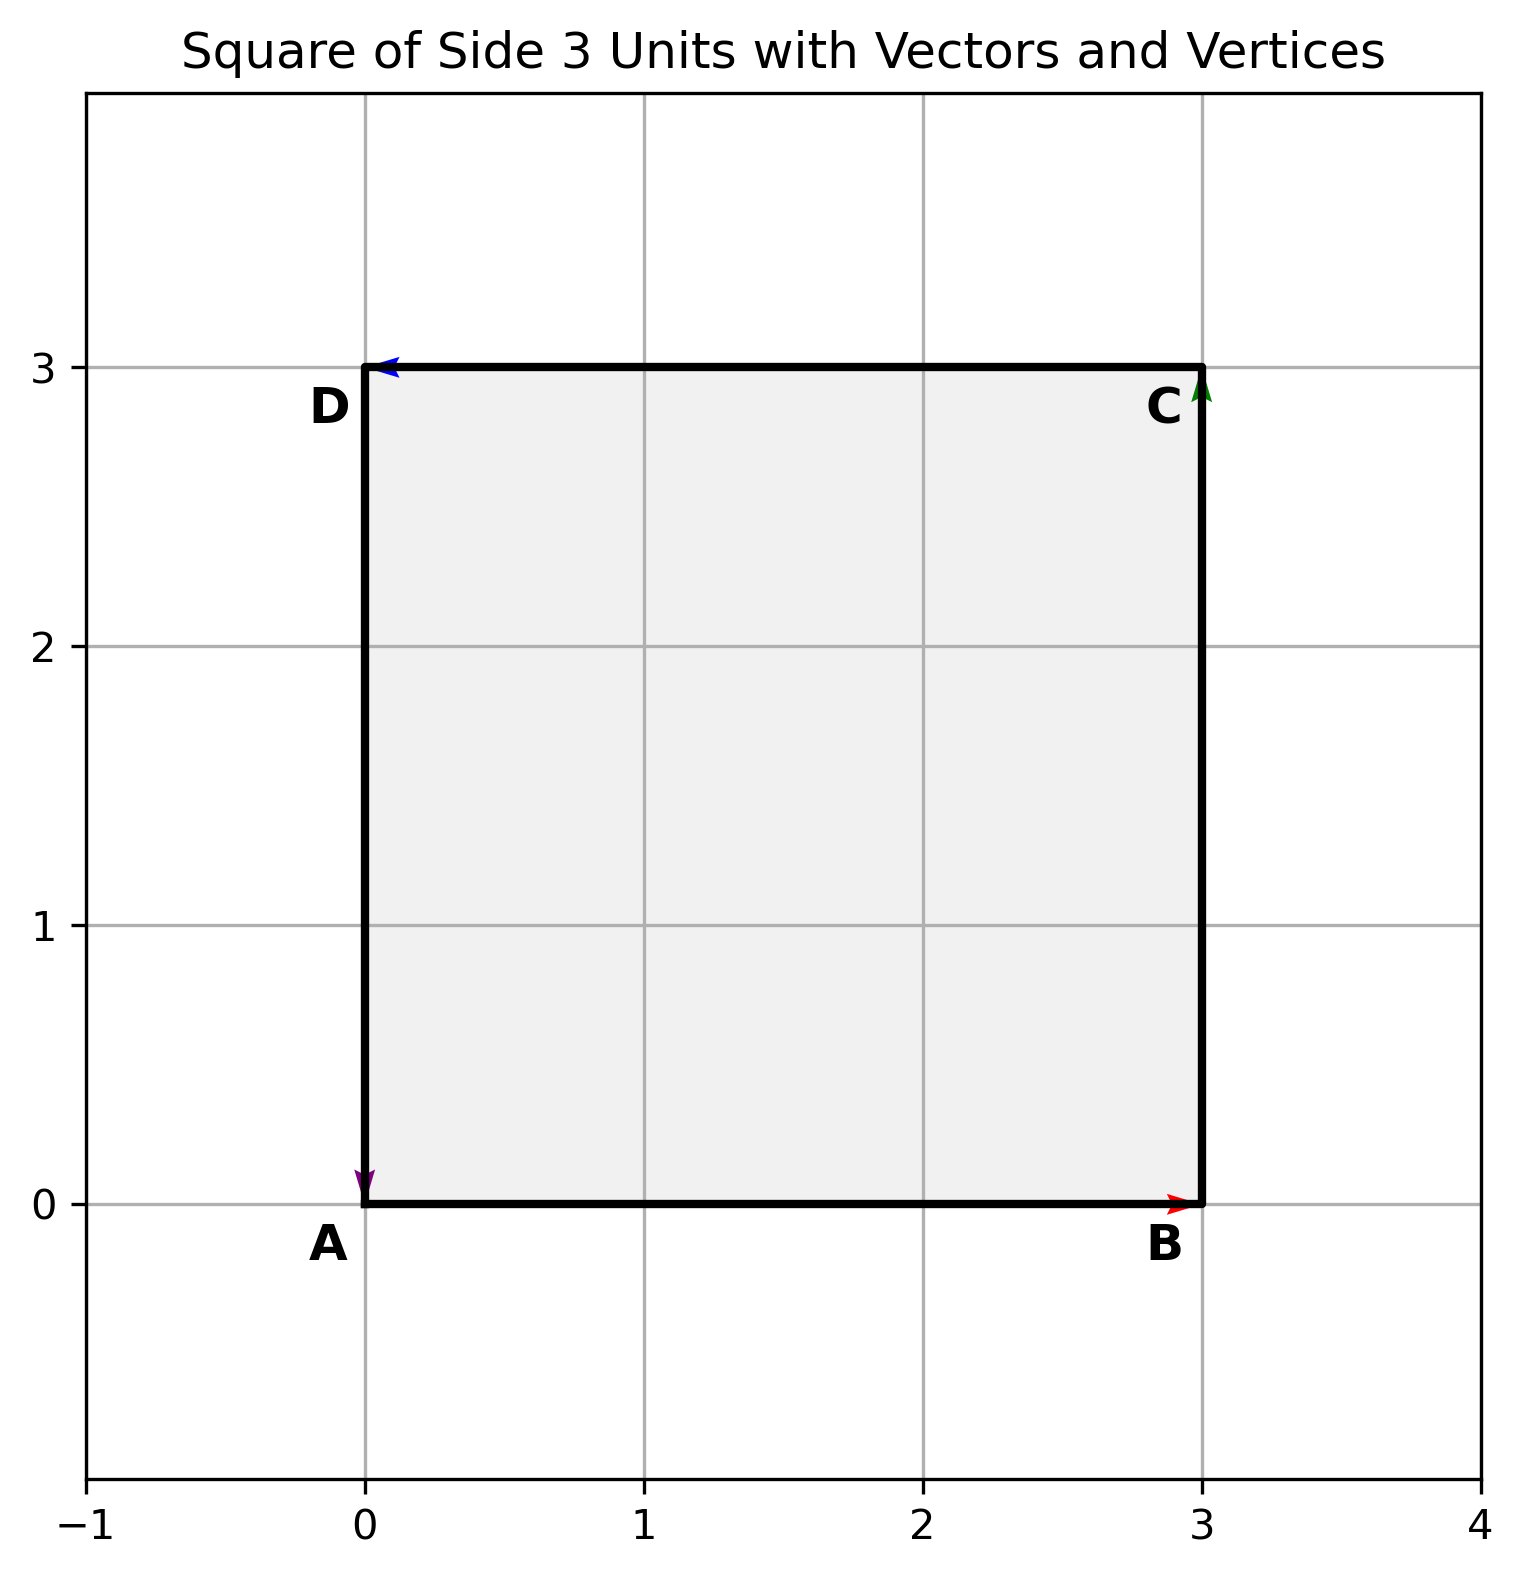
\includegraphics[width=0.5\linewidth]{figures/square_plot.png}
    \caption{Caption}
    \label{square}
\end{figure}

\newpage
\textbf{\Large Properties of square}\\
\begin{enumerate}
    \item All sides have equal length
    \item Opposite sides are parallel
    \item Diagonals have equal length
    \item Adjecent sides are perpendicular to each other


    \begin{align}
        \norm{\Vec{A}-\Vec{B}}= \norm{\Vec{B}-\Vec{C}}= \norm{\Vec{C}-\Vec{D}}= \norm{\Vec{D}-\Vec{A}}
    \end{align}
    \begin{align}
        \Vec{A}-\Vec{B}=\Vec{D}-\Vec{C}
    \end{align}
    \begin{align}
         \norm{\Vec{A}-\Vec{C}}= \norm{\Vec{B}-\Vec{D}}
    \end{align}
    \begin{align}
        (\Vec{A}-\Vec{B})^T(\Vec{B}-\Vec{C})=(\Vec{B}-\Vec{C})^T(\Vec{C}-\Vec{D})=(\Vec{C}-\Vec{D})^T(\Vec{D}-\Vec{A})=(\Vec{D}-\Vec{A})^T(\Vec{A}-\Vec{B})=0
\end{align}
\end{enumerate}
\end{document}
